% This is samplepaper.tex, a sample chapter demonstrating the
% LLNCS macro package for Springer Computer Science proceedings;
% Version 2.21 of 2022/01/12
%
\documentclass[runningheads]{llncs}
%
\usepackage[T1]{fontenc}
% T1 fonts will be used to generate the final print and online PDFs,
% so please use T1 fonts in your manuscript whenever possible.
% Other font encondings may result in incorrect characters.


% tightlist command for lists without linebreak
\providecommand{\tightlist}{%
  \setlength{\itemsep}{0pt}\setlength{\parskip}{0pt}}


% Pandoc citation processing
\newlength{\cslhangindent}
\setlength{\cslhangindent}{1.5em}
\newlength{\csllabelwidth}
\setlength{\csllabelwidth}{3em}
\newlength{\cslentryspacingunit} % times entry-spacing
\setlength{\cslentryspacingunit}{\parskip}
% for Pandoc 2.8 to 2.10.1
\newenvironment{cslreferences}%
  {}%
  {\par}
% For Pandoc 2.11+
\newenvironment{CSLReferences}[2] % #1 hanging-ident, #2 entry spacing
 {% don't indent paragraphs
  \setlength{\parindent}{0pt}
  % turn on hanging indent if param 1 is 1
  \ifodd #1
  \let\oldpar\par
  \def\par{\hangindent=\cslhangindent\oldpar}
  \fi
  % set entry spacing
  \setlength{\parskip}{#2\cslentryspacingunit}
 }%
 {}
\usepackage{calc}
\newcommand{\CSLBlock}[1]{#1\hfill\break}
\newcommand{\CSLLeftMargin}[1]{\parbox[t]{\csllabelwidth}{#1}}
\newcommand{\CSLRightInline}[1]{\parbox[t]{\linewidth - \csllabelwidth}{#1}\break}
\newcommand{\CSLIndent}[1]{\hspace{\cslhangindent}#1}

\usepackage{hyperref}
\hypersetup{colorlinks = TRUE,  urlcolor = blue, linkcolor = blue, citecolor = blue}


\usepackage{graphicx}
% Used for displaying a sample figure. If possible, figure files should
% be included in EPS format.
%
% If you use the hyperref package, please uncomment the following two lines
% to display URLs in blue roman font according to Springer's eBook style:
\usepackage{hyperref}
\usepackage{color}
\renewcommand\UrlFont{\color{blue}\rmfamily}


\begin{document}


\title{biclaR: Estimating the socio-environmental impacts of car
substitution by bicycle and public transit using open tools}
%
\titlerunning{biclaR: SE impacts of car substitution by bicycle and
public transit}
% If the paper title is too long for the running head, you can set
% an abbreviated paper title here
%
\author{Rosa Félix\inst{1}\orcidID{0000-0002-5642-6006} \and Filipe
Moura\inst{1}\orcidID{0000-0001-7749-8490} \and Robin
Lovelace\inst{2}\orcidID{0000-0001-5679-6536}}


\authorrunning{R. Félix et al.}
% First names are abbreviated in the running head.
% If there are more than two authors, 'et al.' is used.
%

\institute{CERIS - Instituto Superior Técnico, University of Lisbon. Av
Rovisco Pais 1049-001 Lisboa, Portugal\\
\email{\href{mailto:rosamfelix@tecnico.ulisboa.pt}{\nolinkurl{rosamfelix@tecnico.ulisboa.pt}}}\\ \and Institute
for Transport Studies, University of Leeds. 34-40 University Rd, Leeds
LS2 9JT, UK}

\maketitle              % typeset the header of the contribution
%
\begin{abstract}
A high proportion of car trips can be replaced by a combination of
public transit and cycling for the first-and-last mile. This paper
estimates the potential for cycling combined with public transit (PT) as
a substitute for car trips in the Lisbon metropolitan area and assesses
its socio-environmental impacts using open data and open source tools. A
decision support tool that facilitates the design and development of a
metropolitan cycling network was developed (\emph{biclaR}). The social
and environmental impacts were assessed using the \emph{HEAT for
Cycling} and the \emph{HEAT as a Service} tools. The impacts of shifting
car trips to PT were also estimated and monetized. The results indicate
that 20\% of car trips could switch to the bicycle + PT combination.
Shifting to cycling for the first-and-last mile stages can reduce annual
CO\textsubscript{2}eq emissions from 6,000 tons/day, with benefits over
10 years of €230 million. For the PT leg, the transfer from car avoids
of at least 8,500 tons of CO\textsubscript{2}eq emissions per year. This
evidence can support policymakers to prioritize interventions that
reduce the reliance on private motor vehicles.

\keywords{Active transport \and Intermodality \and First and last
mile \and Health economic assessment \and Environmental
impacts \and Open data and methods}

\end{abstract}

\hypertarget{introduction}{%
\section{Introduction}\label{introduction}}

Combining public transportation (PT) and cycling for the first and last
mile in metropolitan areas can significantly replace private car trips.
This approach requires interventions and programs to make bicycling more
appealing, and the resulting public investments can have significant
social and environmental benefits.

According to the latest mobility survey conducted in 2018 {[}1{]}, the
LMA registered a total of 5.3 million daily trips, with only 0.5\% by
bicycle. Car modal share was 58.4\%, while PT accounted for 15.5\%. The
number of intra-municipal trips --- with origin and destination in the
same municipality --- amounts to 3.5 million trips. This exceeds the
number of inter-municipal trips (1.8 million trips), involving travel
between different municipalities. Cars and public transport are the most
used modes for intercity trips, with cars being the predominant choice
for all journeys.

To achieve the cycling targets set by the Portuguese national cycling
strategy for 2025 and 2030 (4\% and 10\%, respectively) {[}2{]}, the
Lisbon's Metropolitan Department of Transport introduced
\emph{biclaR}\footnote{See
  \href{https://biclar.tmlmobilidade.pt/}{biclar.tmlmobilidade.pt}}, a
decision support tool that facilitates the design and development of a
metropolitan cycling network {[}3{]}.

\emph{biclaR} builds on the Propensity to Cycle Tool\footnote{See
  \href{https://www.pct.bike/}{pct.bike}} (PCT), a web application and
research project funded by the UK's Department for Transport in 2015
which launched nationally in 2017 as part of the government's Cycling
and Walking Investment Strategy. The PCT initially used only
origin-destination data for commuting trips as the basis of estimates of
cycling potential at zone, route and route network levels {[}4{]}. The
PCT has been extended to include cycling potential for travel to school
in England {[}5{]} and other trip types in other countries.\footnote{See
  \href{https://www.npt.scot}{npt.scot} and
  \href{https://cruse.bike}{cruse.bike} for examples of the PCT in
  Scotland and Ireland that include estimates of cycling for other
  purposes.} However, to the best of our knowledge, this is the first
time that the method has been integrated with public transport data
using multi-modal routing to estimate the potential and benefits of
multi-stage cycling and PT trips.

This paper estimates the potential for combining cycling and PT to
substitute car trips in the LMA. After presenting the methods used, it
assesses its socio-environmental impacts using open data and open-source
tools.

\hypertarget{methods}{%
\section{Methods}\label{methods}}

\hypertarget{modeling-origin-destination-trips}{%
\subsection{Modeling Origin-Destination
trips}\label{modeling-origin-destination-trips}}

The mobility survey data {[}1{]} is the basis for this project and
defines the baseline scenario. Despite being conducted in the
pre-pandemic period (2017), this dataset represents the most
comprehensive and up-to-date information on urban mobility in Portuguese
metropolitan areas (Lisbon and Porto).

We used a method for disaggregating the origins and destinations of
trips between the centroids of two districts (same as ``parish'') to
ensure that a district is not solely characterized by a single point of
origin and destination for its trips. Aggregating all trips into
centroids renders the exercise less realistic, as it excludes a
significant portion of short-distance trips, a prevalent characteristic
of active mode travel {[}6{]}. The OD Jittering method breaks down a
single point (i.e., the centroid of an area) into multiple random points
on the existing and neighboring road network, using OpenStreetMap as a
reference. This method then distributes the volume of trips within the
district among the randomly generated origin-destination pairs.

Using the
\href{https://github.com/dabreegster/odjitter}{\texttt{odjitter} R
package}, we employed a maximum disaggregation level of 100 trips per
O-D pair for this project. Figure \ref{fig:jitter} illustrates the
contrast between trip representation through the traditional method,
which connects a single desire line between each district, and the
presentation achieved through the randomization and disaggregation of
trips between districts, specifically for the Lisbon metropolitan area.

\begin{figure}

{\centering 
\includegraphics[width=1\linewidth,]{img/jitter} 

}

\caption{Representation of OD pairs in the Lisbon metropolitan area between districts, without jittering (left) and with jittering (right).}\label{fig:jitter}
\end{figure}

Although this method provides a more realistic representation of the
trips undertaken compared to the traditional approach, it does not fully
align with the actual O-D pairs of trips, which remain unknown due to
data privacy regulations.

\hypertarget{modeling-routes}{%
\subsection{Modeling routes}\label{modeling-routes}}

The mobility survey collects the origin and destination of trips but
does not include the respective routes. Modeling the realistic cycling +
PT routes between OD pairs depends on assumptions regarding the
characteristics of the cycling and road networks and the location of
public transport interfaces. Other constraints regarding the behavior of
potential cyclists determine the routing results. For example, such
restrictions can favor low speed, low traffic streets, more direct
routes, and less steep paths, among others, suitable for cycling.

The selected route choice algorithm was the
\href{https://ipeagit.github.io/r5r/}{\texttt{r5r} R package} {[}7{]},
which allows for great flexibility in configuring estimated route types,
and which proven to provide most accurate route networks for the city of
Lisbon {[}8{]}. \texttt{r5r} can calculate multi-modal routes using PT
combined with other modes. It enables the identification of the most
direct or safest cycling routes, using the Level of Traffic
Stress\footnote{see
  \href{https://docs.conveyal.com/learn-more/traffic-stress}{docs.conveyal.com/learn-more/traffic-stress}}
(LTS) scale, ranging from 1 to 4, where 1 corresponds to the quietest
(e.g., off-road cycle paths) and 4 corresponds to the least quiet (e.g.,
routes shared with motorized traffic). The routes were estimated for the
base scenario for both types of networks: \emph{direct} and \emph{safe},
using LTS 4 and LTS 3, respectively.

The \texttt{r5r} model used the OpenStreetMap road network and the GTFS
metropolitan data agregated and validated. This information is crucial
for an accurate PT trip and route estimation. A digital elevation model
from the European Space Agency's COPERNICUS mission, with a 25m spatial
resolution, was used to include street gradient information, as a weight
in cycling routing. The cycling potential trips for the two national
strategic targets (4\% and 10\%) was estimated from the values for
cycling and car trips (both as a driver and as a passenger) from the
2017 base scenario.

The routes were then overlaid and aggregated by segments, using
\href{https://docs.ropensci.org/stplanr/reference/overline.html}{\texttt{stplanr\ overline()}
R function}.

\hypertarget{modeling-intermodality}{%
\subsection{Modeling intermodality}\label{modeling-intermodality}}

The intermodality scenario considers trips combining PT and cycling for
the first and last legs. In a conservative approach, we have restricted
our analysis to the first and last legs with a combined length of up to
5 km or up to 25 minutes on bike. Furthermore, we have imposed
restrictions on PT usage to include only trips with no PT transfers, and
up to 2 hours (120 min). Additionally, we have only included PT modes
that can easily accommodate bicycles, such as trains, ferries, trams,
and inter-municipal bus lines equipped with bike racks (Figure
\ref{fig:map1}).

\begin{figure}

{\centering 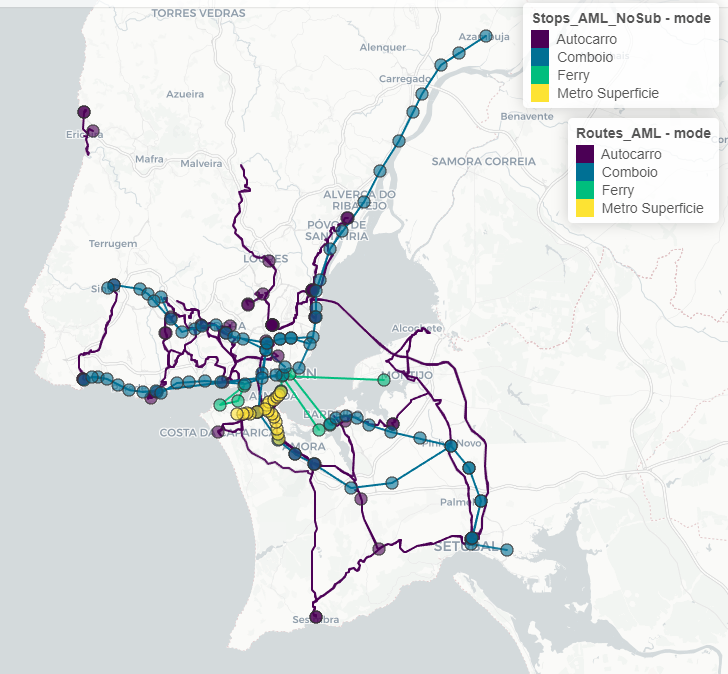
\includegraphics[width=0.6\linewidth,]{img/map1} 

}

\caption{Interfaces and lines considered, by transport mode, in the Lisbon metropolitan area}\label{fig:map1}
\end{figure}

Figure \ref{fig:map2} illustrates the resulting bicycle routes to access
the main PT interfaces in the LMA.

\begin{figure}

{\centering 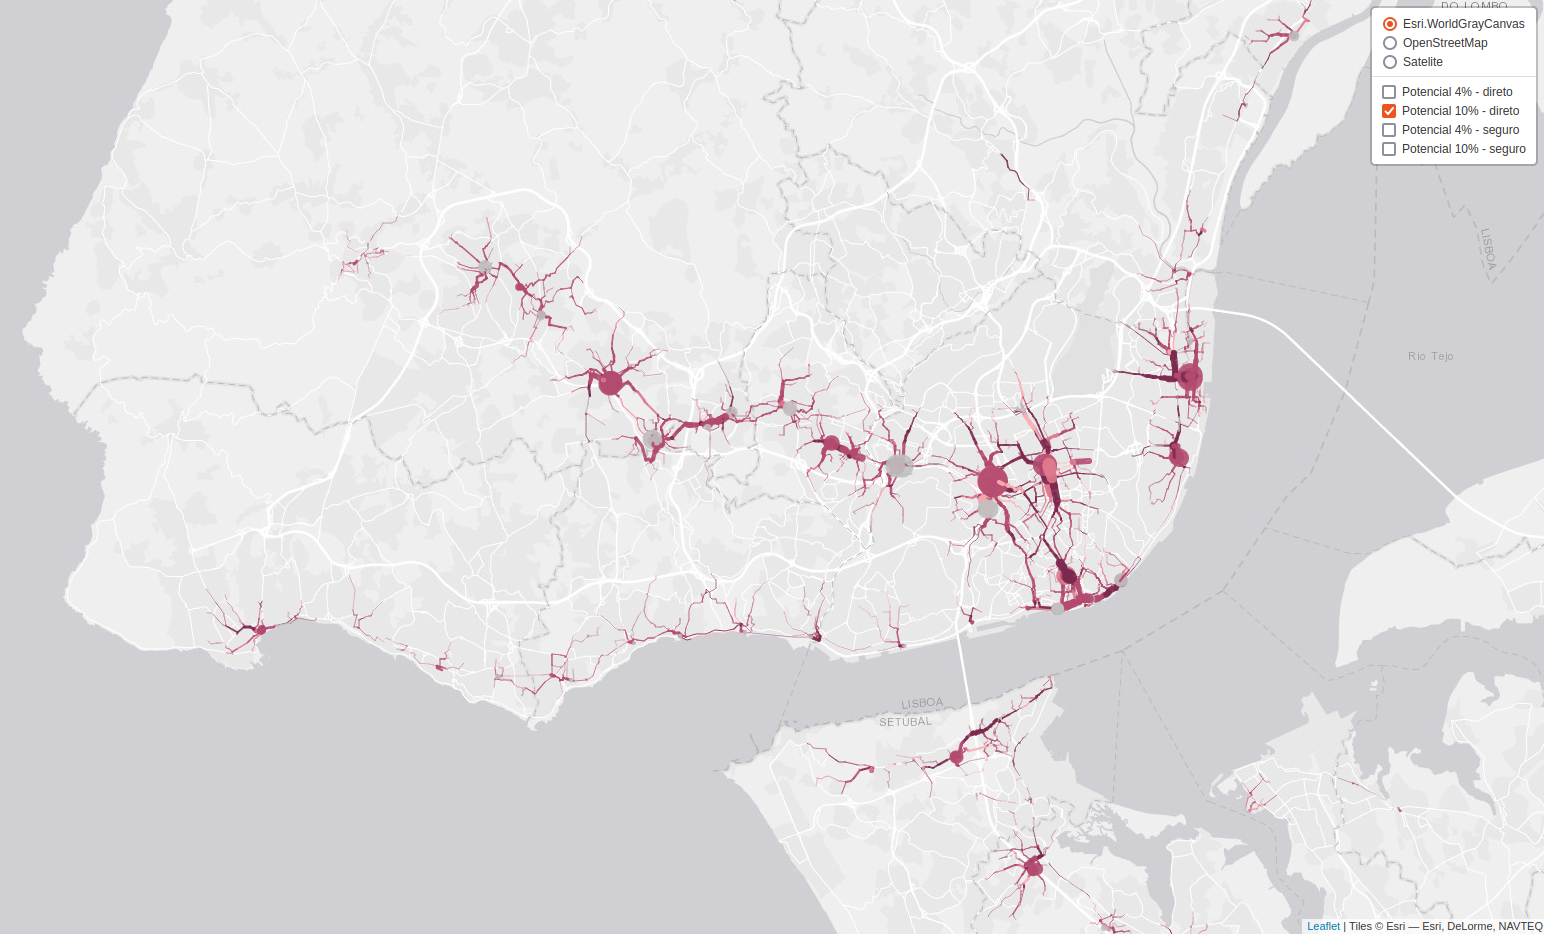
\includegraphics[width=0.8\linewidth,]{img/map2} 

}

\caption{Bike routes with highest potential to serve as first and last leg when replacing cycling and PT from car trips (screenshot of the interactive online tool).}\label{fig:map2}
\end{figure}

\hypertarget{assessing-socio-environmental-benefits---continue-from-here}{%
\subsection{Assessing socio-environmental benefits - CONTINUE FROM
HERE}\label{assessing-socio-environmental-benefits---continue-from-here}}

Socio-environmental impacts were estimated for a short term time horizon
(i.e., one year) and the long term (i.e., ten years). using the HEAT for
Cycling and the HEAT as a Service\footnote{see
  \url{https://github.com/HEAT-WHO/HEAT_heatr_api}} tools, from the WHO.

Os impactes foram avaliados para cada cenário e para diferentes escalas
territoriais:

\begin{itemize}
\tightlist
\item
  Desagregado à escala municipal para cada segmento de rede:

  \begin{itemize}
  \tightlist
  \item
    Ambientais (emissões de CO\textsubscript{2}eq evitadas);
  \item
    Balanço monetarizado dos impactes socioeconómicos totais
    (considerando o balanço dos impactes ambientais e sociais);
  \end{itemize}
\item
  Agregado à escala metropolitana:

  \begin{itemize}
  \tightlist
  \item
    Ambientais (emissões de CO\textsubscript{2}eq evitadas);
  \item
    Balanço monetarizado dos impactes socioeconómicos totais
    (considerando o balanço dos impactes ambientais e sociais);
  \item
    Ambientais (emissões de CO\textsubscript{2}eq, CO, PM10, NOx, e
    VOC11, evitadas por substituição dos modos motorizados, considerando
    as emissões geradas na transferência para transportes públicos).
  \end{itemize}
\end{itemize}

Para todos os cenários, recorreu-se à ferramenta HEAT for cycling, da
Organização Mundial de Saúde, para estimativa dos impactes sociais e
ambientais da transferência de viagens em automóvel para viagens em
bicicleta, nas componentes de: a) Social - Saúde, Atividade Física,
Exposição a poluição atmosférica, Exposição ao risco de sinistralidade
rodoviária; b) Ambiental - Emissão de gases CO\textsubscript{2}eq.

Additionally, we estimate the impacts of shifting car trips to PT for
the second leg of the journey with EMEP/EEA's COPERT methodology and
monetize them with the EU Guide to cost-benefit analysis.

A estimativa dos impactes ambientais resulta em toneladas de
CO\textsubscript{2}eq, e a estimativa dos impactes sociais resulta em
mortalidade prematura evitada. Ambas as unidades são por fim monetizadas
em €, segundo os valores da literatura utilizada em estudos semelhantes.
Para além dos impactes sociais e ambientais resultantes da transferência
do automóvel para a bicicleta (na primeira e na última parte da viagem,
de e para a interface de TP), estimou-se também o impacte ambiental
adicional, resultante da transferência do automóvel para os vários
transportes públicos (na segunda etapa da viagem, entre as interfaces).
Como tal, foi necessário caracterizar o universo dos modos motorizados a
serem considerados para os cálculos dos respetivos fatores de emissões
de gases poluentes e atmosféricos.

Os fatores de consumo e de emissão dos automóveis e transportes públicos
deve ser tido em conta relativamente ao número de passageiros
transportados (por passageiro.km) e não ao veículo (que seria
veículo.km). No caso do automóvel, para contabilizar a emissão de gases
evitados pela transferência de viagens em automóvel para os transportes
públicos, teve-se em conta o valor de referência de 1.61
passageiros/automóvel reportados pelo Inquérito à Mobilidade (INE 2017).

As emissões evitadas por cada viagem em transportes públicos que
substitui o automóvel correspondem às emissões equivalentes de um
automóvel com características correspondentes à média da frota em
circulação em Lisboa, para 2 tipos de combustível: gasolina e gasóleo.
Utilizou-se a metodologia e valores de referência do software COPERT
(Ntziachristos and Samaras 2020), v5.0, da Agência Europeia do Ambiente,
para um nível de detalhe 3 (Tier 3) na estimativa de consumo de emissões
para o automóvel, nestes dois tipos de combustível. Optou-se por usar um
veículo de dimensão familiar, norma EURO, e tipo de combustível gasolina
ou diesel. Considerou-se que as viagens foram todas realizadas em
condições urbanas (com as respetivas implicações no regime médio de
condução) e a uma velocidade média de 15km/h, nos períodos de hora de
ponta. Uma vez que a distância média percorrida por viagem influencia o
nível de sobreconsumo e emissões decorrentes da operação do motor a frio
-- ou seja, distâncias maiores diluem a importância deste sobreconsumo
face ao fator de consumo com o motor a operar a quente, foram estimados
os consumos para diferentes gamas de viagem, em intervalos de 500
metros. As emissões são estimadas para os seguintes poluentes
atmosféricos: CO (monóxido de carbono), NO X (Óxidos de Azoto), COV
(Compostos Orgânicos Voláteis), PM (material particulado). Também é
estimada as emissões dos principais gases com efeito de estufa: CO2
(dióxido de carbono); CH4 (metano) e N2O (Óxido nitroso), assim como o
CO\textsubscript{2}eq equivalente.

Relativamente aos transportes públicos, recorreu-se aos fatores de
emissão reportados nos relatórios de sustentabilidade dos respetivos
operadores (Carris 2020; Metropolitano de Lisboa 2020; CP 2020, Grupo
Transtejo 2014).

a conversão das emissões evitadas em perda de bem-estar evitado, através
da respetiva valorização monetária. a partir dos valores de referência
para os vários gases contabilizados, atualizados para 2022 15, com base
nas fontes: Bickel et al.~(2006), Nash and others (2003), Sartori et
al.~(2014).

\hypertarget{results-and-discussion}{%
\section{Results and Discussion}\label{results-and-discussion}}

A Tabela 4 apresenta o número de viagens diárias do cenário base e
potenciais, passíveis de serem realizadas até 5 km em bicicleta em
complemento com TP, por tipo de percurso. Para as redes segura e direta,
as viagens do cenário base até 5 km em bicicleta + TP correspondem a
20\% do total de viagens reportadas no inquérito.

Este cenário valoriza a utilização da bicicleta como complemento ao
transporte público, com potencial de aumentar as viagens em TP
realizadas na área metropolitana de Lisboa em até 12\% (acrescentando às
825 mil do IMob 2017). Estes resultados sugerem que o potencial de
transferência de viagens em automóvel para bicicleta + TP poderá ser
quase ou tão importante quanto a transferência para viagens utilizando
apenas a bicicleta.

Para este cenário foram estimados os impactes ambientais de
transferência do automóvel para os transportes públicos, para além dos
impactes ambientais e sociais da transferência para a bicicleta

Foram então calculadas as emissões dos poluentes para cada viagem
substituída, tendo em conta o modo de transporte, distâncias e
velocidade. A tabela 11 apresenta a estimativa anual de gases emitidos e
evitados por transferência do automóvel para os outros modos de
transporte público, como exemplo para o cenário com a meta de 4\%,
usando a rede ciclável ``direta''.

\[Tabela 11\]

Para esse cenário com essas características, é estimada uma poupança de
8 702 toneladas de CO\textsubscript{2}eq por via da transferência de
viagens motorizadas com combustíveis fósseis e eletricidade, numa
perspetiva de ciclo de vida da produção de eletricidade.

A valorização monetária das emissões (em toneladas) é apresentada na
tabela seguinte, para o cenário 3 (apenas a segunda parte da viagem, em
transportes públicos), com as metas de 4\% e 10\%, e usando as redes
cicláveis ``direta'' e ``segura'', para 365 dias (1 ano).

\[Tabela 13\]

\begin{figure}
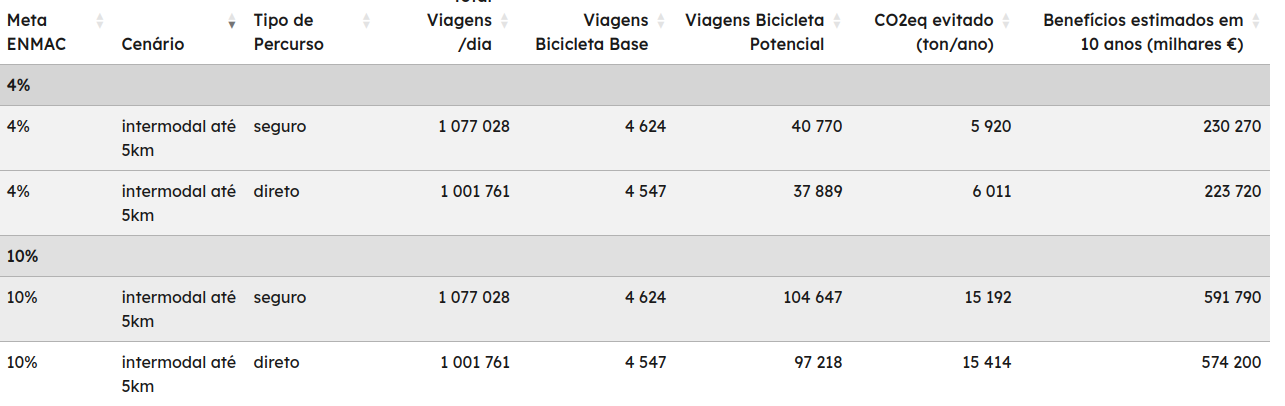
\includegraphics[width=1\linewidth,]{img/table1} \caption{Summary of the cycling potencial of intermodality scenario.}\label{fig:summary1}
\end{figure}

\begin{figure}
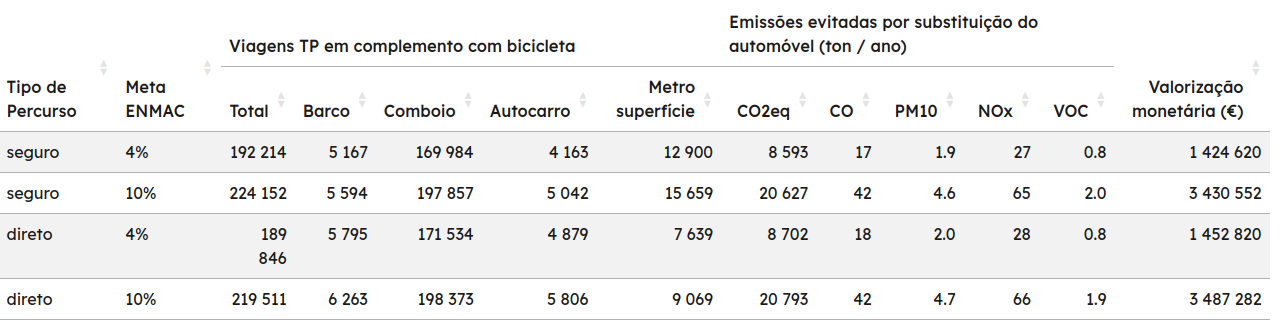
\includegraphics[width=1\linewidth,]{img/table2} \caption{Potencial de transferência estimado para cada modo de transporte público, bem como as estimativas de consumo de CO~2~eq evitado anualmente por transferência do automóvel.}\label{fig:summary2}
\end{figure}

Em suma, o impacte socioeconómico das emissões de gases poluentes e de
gases de efeito estufa pode ser valorizado numa poupança potencial de
entre 1.4 a 3.5 milhões €, a acrescentar aos impactes estimados na
secção anterior.

The results indicate that 20\% of the current trips can be made with the
bicycle + PT combination, with an additional 12\% of PT trips being
potentially replaced. Shifting to cycling for the first-and-last mile
can reduce annual CO\textsubscript{2}eq emissions by 6,000 to 15,000
tons/day, and the 10-year socio-environmental benefits account for €230
to €590 million, depending on the cycling targets. For the PT leg, the
transfer from car results in the avoidance of 8,500 to 20,800 tons of
CO\textsubscript{2}eq emissions per year, or €1.4 to €3.5 million over
10 years, with trains offering the greatest potential for substitution
(88\%).

\hypertarget{conclusion}{%
\section{Conclusion}\label{conclusion}}

By making the research process publicly accessible in a code repository,
this study enables the replication of similar estimates for
socio-environmental impacts resulting from a modal shift from cars to
bicycles + PT in other metropolitan areas.

The train with most potential (as seen from fig 2)

The information available at the open access website can be downloaded,
and used with any GIS software to, for instance, understant which
cycling connections have the highest socioenvironmental impacts, in tons
of avoided CO2eq emissions, or in long term social costs.

The provided information on socio-economic benefits can support
policymakers in prioritizing interventions to reduce the reliance on
individual motorized transportation and effectively communicate their
decisions.

\hypertarget{acknowledgements}{%
\subsubsection*{Acknowledgements}\label{acknowledgements}}
\addcontentsline{toc}{subsubsection}{Acknowledgements}

Thomas Götshi - HAAS.

\hypertarget{references}{%
\section*{References}\label{references}}
\addcontentsline{toc}{section}{References}

\hypertarget{refs}{}
\begin{CSLReferences}{0}{0}
\leavevmode\vadjust pre{\hypertarget{ref-IMOB}{}}%
\CSLLeftMargin{1. }%
\CSLRightInline{INE: Mobilidade e funcionalidade do território nas
{Áreas Metropolitanas do Porto e de Lisboa}: 2017,
\url{https://www.ine.pt/xportal/xmain?xpid=INE\&xpgid=ine_publicacoes\&PUBLICACOESpub_boui=349495406\&PUBLICACOESmodo=2\&xlang=pt},
(2018).}

\leavevmode\vadjust pre{\hypertarget{ref-ENMAC}{}}%
\CSLLeftMargin{2. }%
\CSLRightInline{Presidência do Conselho de Ministros: Resolução do
conselho de ministros n.º 131/2019,
\url{https://files.dre.pt/1s/2019/08/14700/0004600081.pdf}, (2019).}

\leavevmode\vadjust pre{\hypertarget{ref-felix2023}{}}%
\CSLLeftMargin{3. }%
\CSLRightInline{Félix, R., Lovelace, R., Moura, F.: {biclaR - Ferramenta
de apoio ao planeamento da rede ciclável na área metropolitana de
Lisboa}, \url{https://biclar.tmlmobilidade.pt}, (2022).}

\leavevmode\vadjust pre{\hypertarget{ref-lovelace2017}{}}%
\CSLLeftMargin{4. }%
\CSLRightInline{Lovelace, R., Goodman, A., Aldred, R., Berkoff, N.,
Abbas, A., Woodcock, J.: The Propensity to Cycle Tool: An open source
online system for sustainable transport planning. Journal of Transport
and Land Use. 10, (2017).
https://doi.org/\href{https://doi.org/10.5198/jtlu.2016.862}{10.5198/jtlu.2016.862}.}

\leavevmode\vadjust pre{\hypertarget{ref-goodman2019}{}}%
\CSLLeftMargin{5. }%
\CSLRightInline{Goodman, A., Rojas, I.F., Woodcock, J., Aldred, R.,
Berkoff, N., Morgan, M., Abbas, A., Lovelace, R.: Scenarios of cycling
to school in england, and associated health and carbon impacts:
Application of the {`}propensity to cycle tool{'}. Journal of Transport
\& Health. 12, 263--278 (2019).
https://doi.org/\href{https://doi.org/10.1016/j.jth.2019.01.008}{10.1016/j.jth.2019.01.008}.}

\leavevmode\vadjust pre{\hypertarget{ref-Lovelace2022Jittering}{}}%
\CSLLeftMargin{6. }%
\CSLRightInline{Lovelace, R., Félix, R., Carlino, D.: Jittering: A
computationally efficient method for generating realistic route networks
from origin-destination data. Findings. (2022).
https://doi.org/\href{https://doi.org/10.32866/001c.33873}{10.32866/001c.33873}.}

\leavevmode\vadjust pre{\hypertarget{ref-r5r}{}}%
\CSLLeftMargin{7. }%
\CSLRightInline{Pereira, R.H.M., Saraiva, M., Herszenhut, D., Braga,
C.K.V., Conway, M.W.: r5r: Rapid realistic routing on multimodal
transport networks with R5 in r. Findings. (2021).
https://doi.org/\href{https://doi.org/10.32866/001c.21262}{10.32866/001c.21262}.}

\leavevmode\vadjust pre{\hypertarget{ref-Lovelace2022exploring}{}}%
\CSLLeftMargin{8. }%
\CSLRightInline{Lovelace, R., Félix, R., Carlino, D.: Exploring
jittering and routing options for converting origin-destination data
into route networks: Towards accurate estimates of movement at the
street level. The International Archives of the Photogrammetry, Remote
Sensing and Spatial Information Sciences. XLVIII-4/W1-2022, 279--286
(2022).
https://doi.org/\href{https://doi.org/10.5194/isprs-archives-XLVIII-4-W1-2022-279-2022}{10.5194/isprs-archives-XLVIII-4-W1-2022-279-2022}.}

\end{CSLReferences}

%
% ---- Bibliography ----



\end{document}
